\chapter[Development of measurements]{Developments in the monitoring network, data quality and database infrastructure}\label{ch:ObsDevel}

{\bf{Wenche Aas, Anne Hjellbrekke and Kjetil T{\o}rseth}}
\vspace{30pt}

\section{\label{sec:Compliance-with-monitoring}Compliance with the EMEP monitoring strategy}

The monitoring obligations of EMEP were updated in 2019 and is defined by the Monitoring Strategy for 2020-2030 (\cite{MonStrat2019}). 

The complexity in the monitoring program with respect to the number of variables and sites, whether parameters are at level 1 or level 2, and the required time resolution (hourly, daily, weekly), makes it challenging to assess whether a country is in compliance. CCC has developed an index to illustrate to what extent the Parties comply, how implementation compares with other countries, and how activities evolve with time.

The index is defined for level 1 parameters only, and is calculated based on the data reported in comparison with the expected. EMEP recommends one site pr 50.000 km$^{2}$, but this target number is adjusted for very large countries (i.e. KZ, RU, TR and UA). The components and number of variables to be measured in accordance to the strategy are as follows: major inorganic ions in precipitation (10 variables), major inorganic components in air (13 variables), ozone (1 variable), PM mass (2 variables) and heavy metals in precipitation (7 variables). For heavy metals, the sampling frequency is weekly, and for the other components it is daily or hourly (ozone). Based on the relative implementation of the different variables, the index has been given the following relative weights: Inorganics in precipitation: 30\%, inorganics in air: 30\%, ozone: 20\%, PM mass: 10\%, heavy metals: 10\%.

Figure~\ref{fig:Index-for-implementation} summarises implementation in 2019 compared to 2000, 2005 and 2010. The countries are sorted from left to right with increasing index for 2019. Slovakia,  Estonia, The Netherlands, Denmark, and Switzerland have almost complete programs with an index of 90\% or higher. Small countries generally comply better (due to more easily satisfying the site density requirements). Since 2010, 35\% of the Parties have improved their monitoring programme,  while 37\% have a decrease. Improvements are seen in e.g. France, Croatia and Belgium.  One Party, Malta, has reported data in 2019 and not in 2010, while Georgia, Moldova, Montenegro and Romania have stopped reporting/measuring. In Figure~\ref{fig:EMEP-measurement-network} in Chapter~\ref{Obs_2019}, the geographical distribution of level 1 sites is shown for 2019.  
In large parts of Europe, implementation of the EMEP monitoring strategy is far from satisfactory. 

\begin{figure}
	\centering
	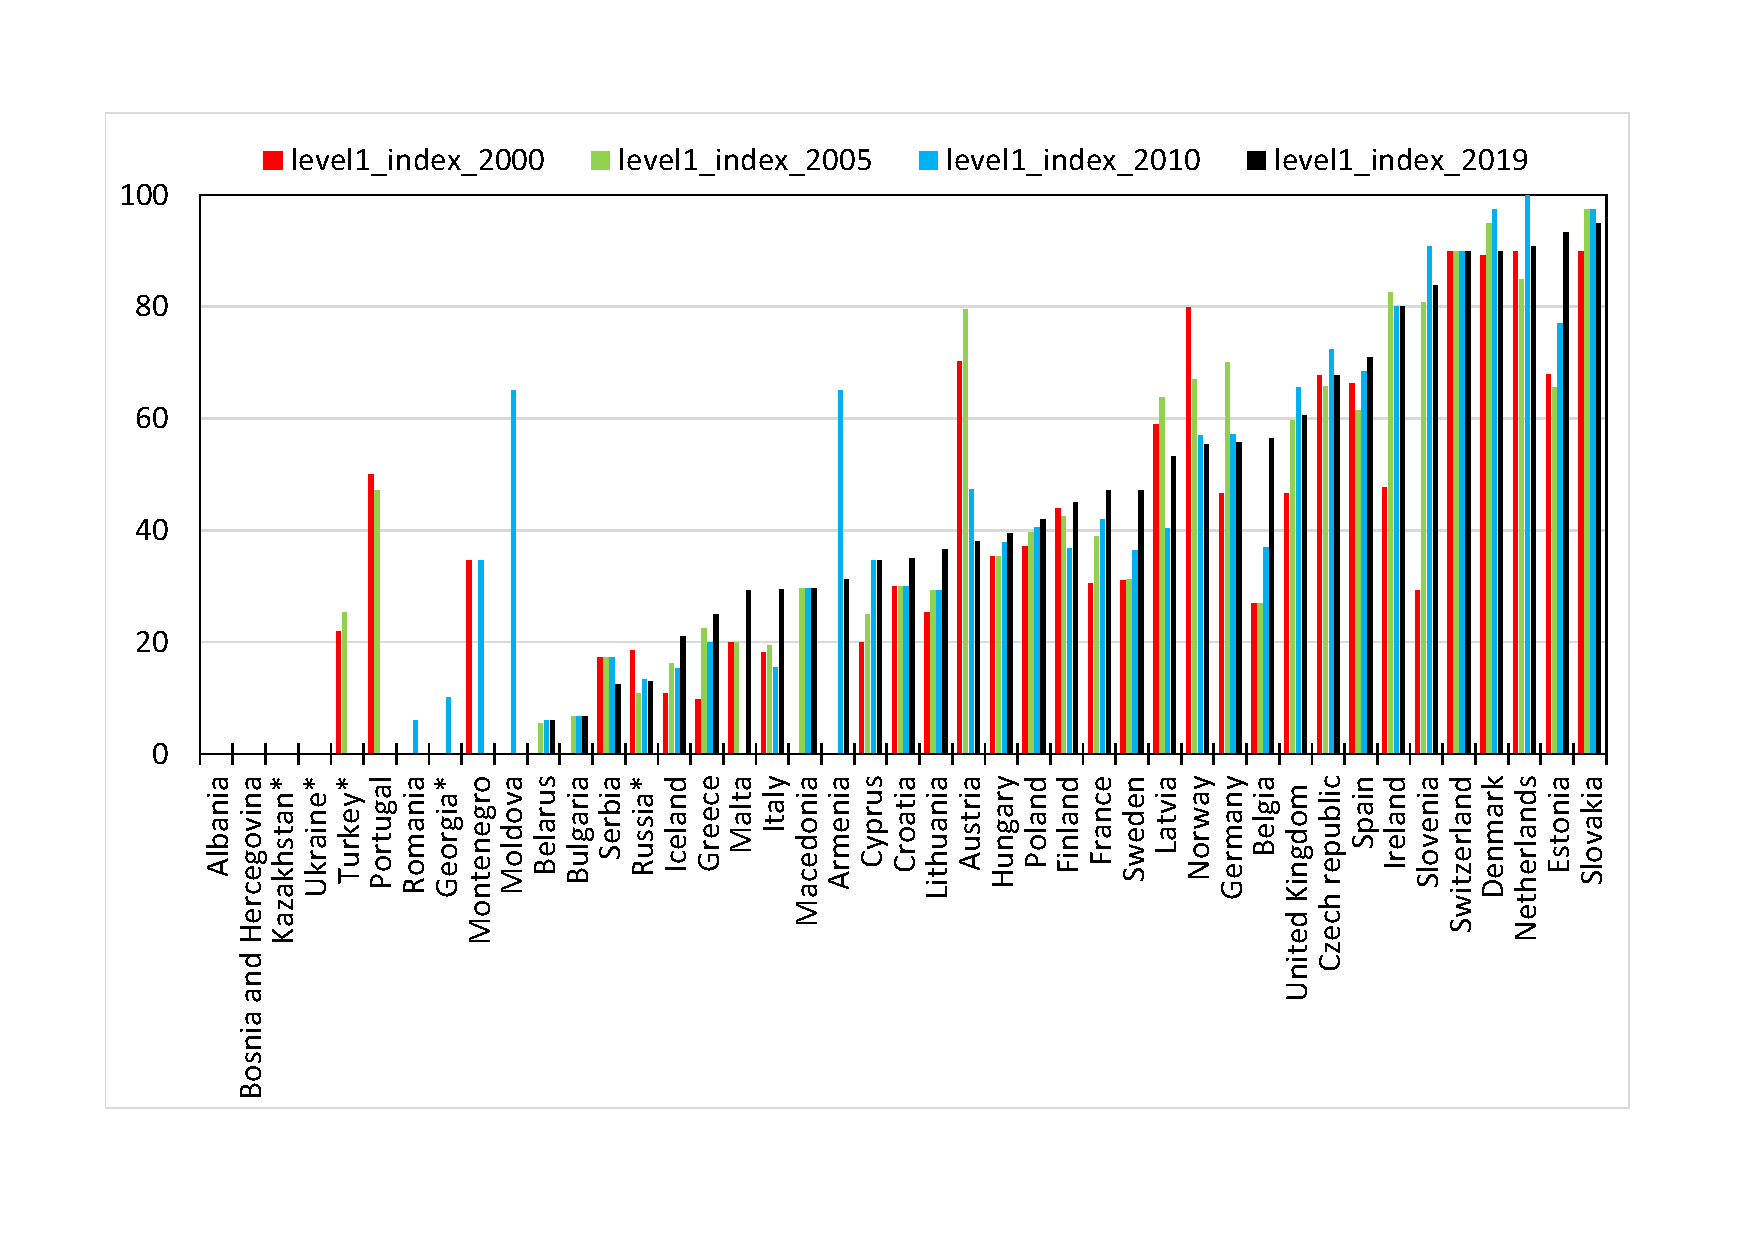
\includegraphics[width=0.74\paperwidth]{FIGS_Obs/index2019.pdf}
	\caption{\label{fig:Index-for-implementation}Index for implementation of the EMEP monitoring strategy, level 1 based on what has been reported for 2000, 2005, 2010 and 2019. {*} means adjusted land area.}
\end{figure}

For the level 2 parameters, an index has not been defined, but mapping the site distribution illustrate the compliance to the monitoring strategy. 56 sites from 21 different Parties reported  at least one of the required  EMEP level 2 parameters relevant to this report (aerosols (50 sites), photo-oxidants (16 sites) and atmospheric tracers (8 sites)). One should note that some of these sites have been reporting data to ACTRIS (the European Research Infrastructure for the observation of Aerosol, Clouds and Trace Gases) and not to EMEP, but they have been included here in the overview since the observations are still comparable with those of EMEP. The sites with measurements of POPs and heavy metals are covered in the EMEP status report published by MSC-E (EMEP Status report 2/2021).  Figure~\ref{fig:levell2-sites} shows that level 2 measurements of aerosols have better spatial coverage than oxidant precursors (VOC + methane) and atmospheric tracers. Few sites have a complete measurement program, and only 12 sites have a complete aerosol program. For oxidant precursors and atmospheric tracers, there are ongoing improvement in the measurement capabilities resulting from development in ACTRIS in co-operation with EMEP and the WMO Global Atmospheric Watch Programme (GAW).

\begin{figure}[h!]
 \centering
  \subfigure[Particulate matter] {\includegraphics*[width=0.3\linewidth]{FIGS_Obs/pm_level_2.png}}
  \subfigure[Oxidant precursors] {\includegraphics*[width=0.3\linewidth]{FIGS_Obs/oxidants.png}}
  \subfigure[Atmospheric tracers] {\includegraphics*[width=0.3\linewidth]{FIGS_Obs/tracer.png}}
\caption{\label{fig:levell2-sites}Sites measuring and reporting EMEP level 2 parameters for the year 2019.}
\end{figure}

\section{Updates in reporting templates and guidelines}

In addition to the requirement that variables has to be measured as defined in the EMEP monitoring 
strategy discussed above, it is important that the data are reported in time to ensure that they can 
be quality assured and included in the database. This allows them to be included in the annual model 
validation, interpretations for the EMEP status reports, as well as other regional assessments and 
studies carried out beyond EMEP.

Figure~\ref{fig:Submission} shows the status of the submission of data for 2019  and to what  extent the data were reported in time. It is obvious that large volumes of data are reported late and some not at all. Of the 33 Parties reporting either level 1 or level 2 data, about  60\% reported within the deadline of 31 July 2020. 

\begin{figure}[h]
\centering
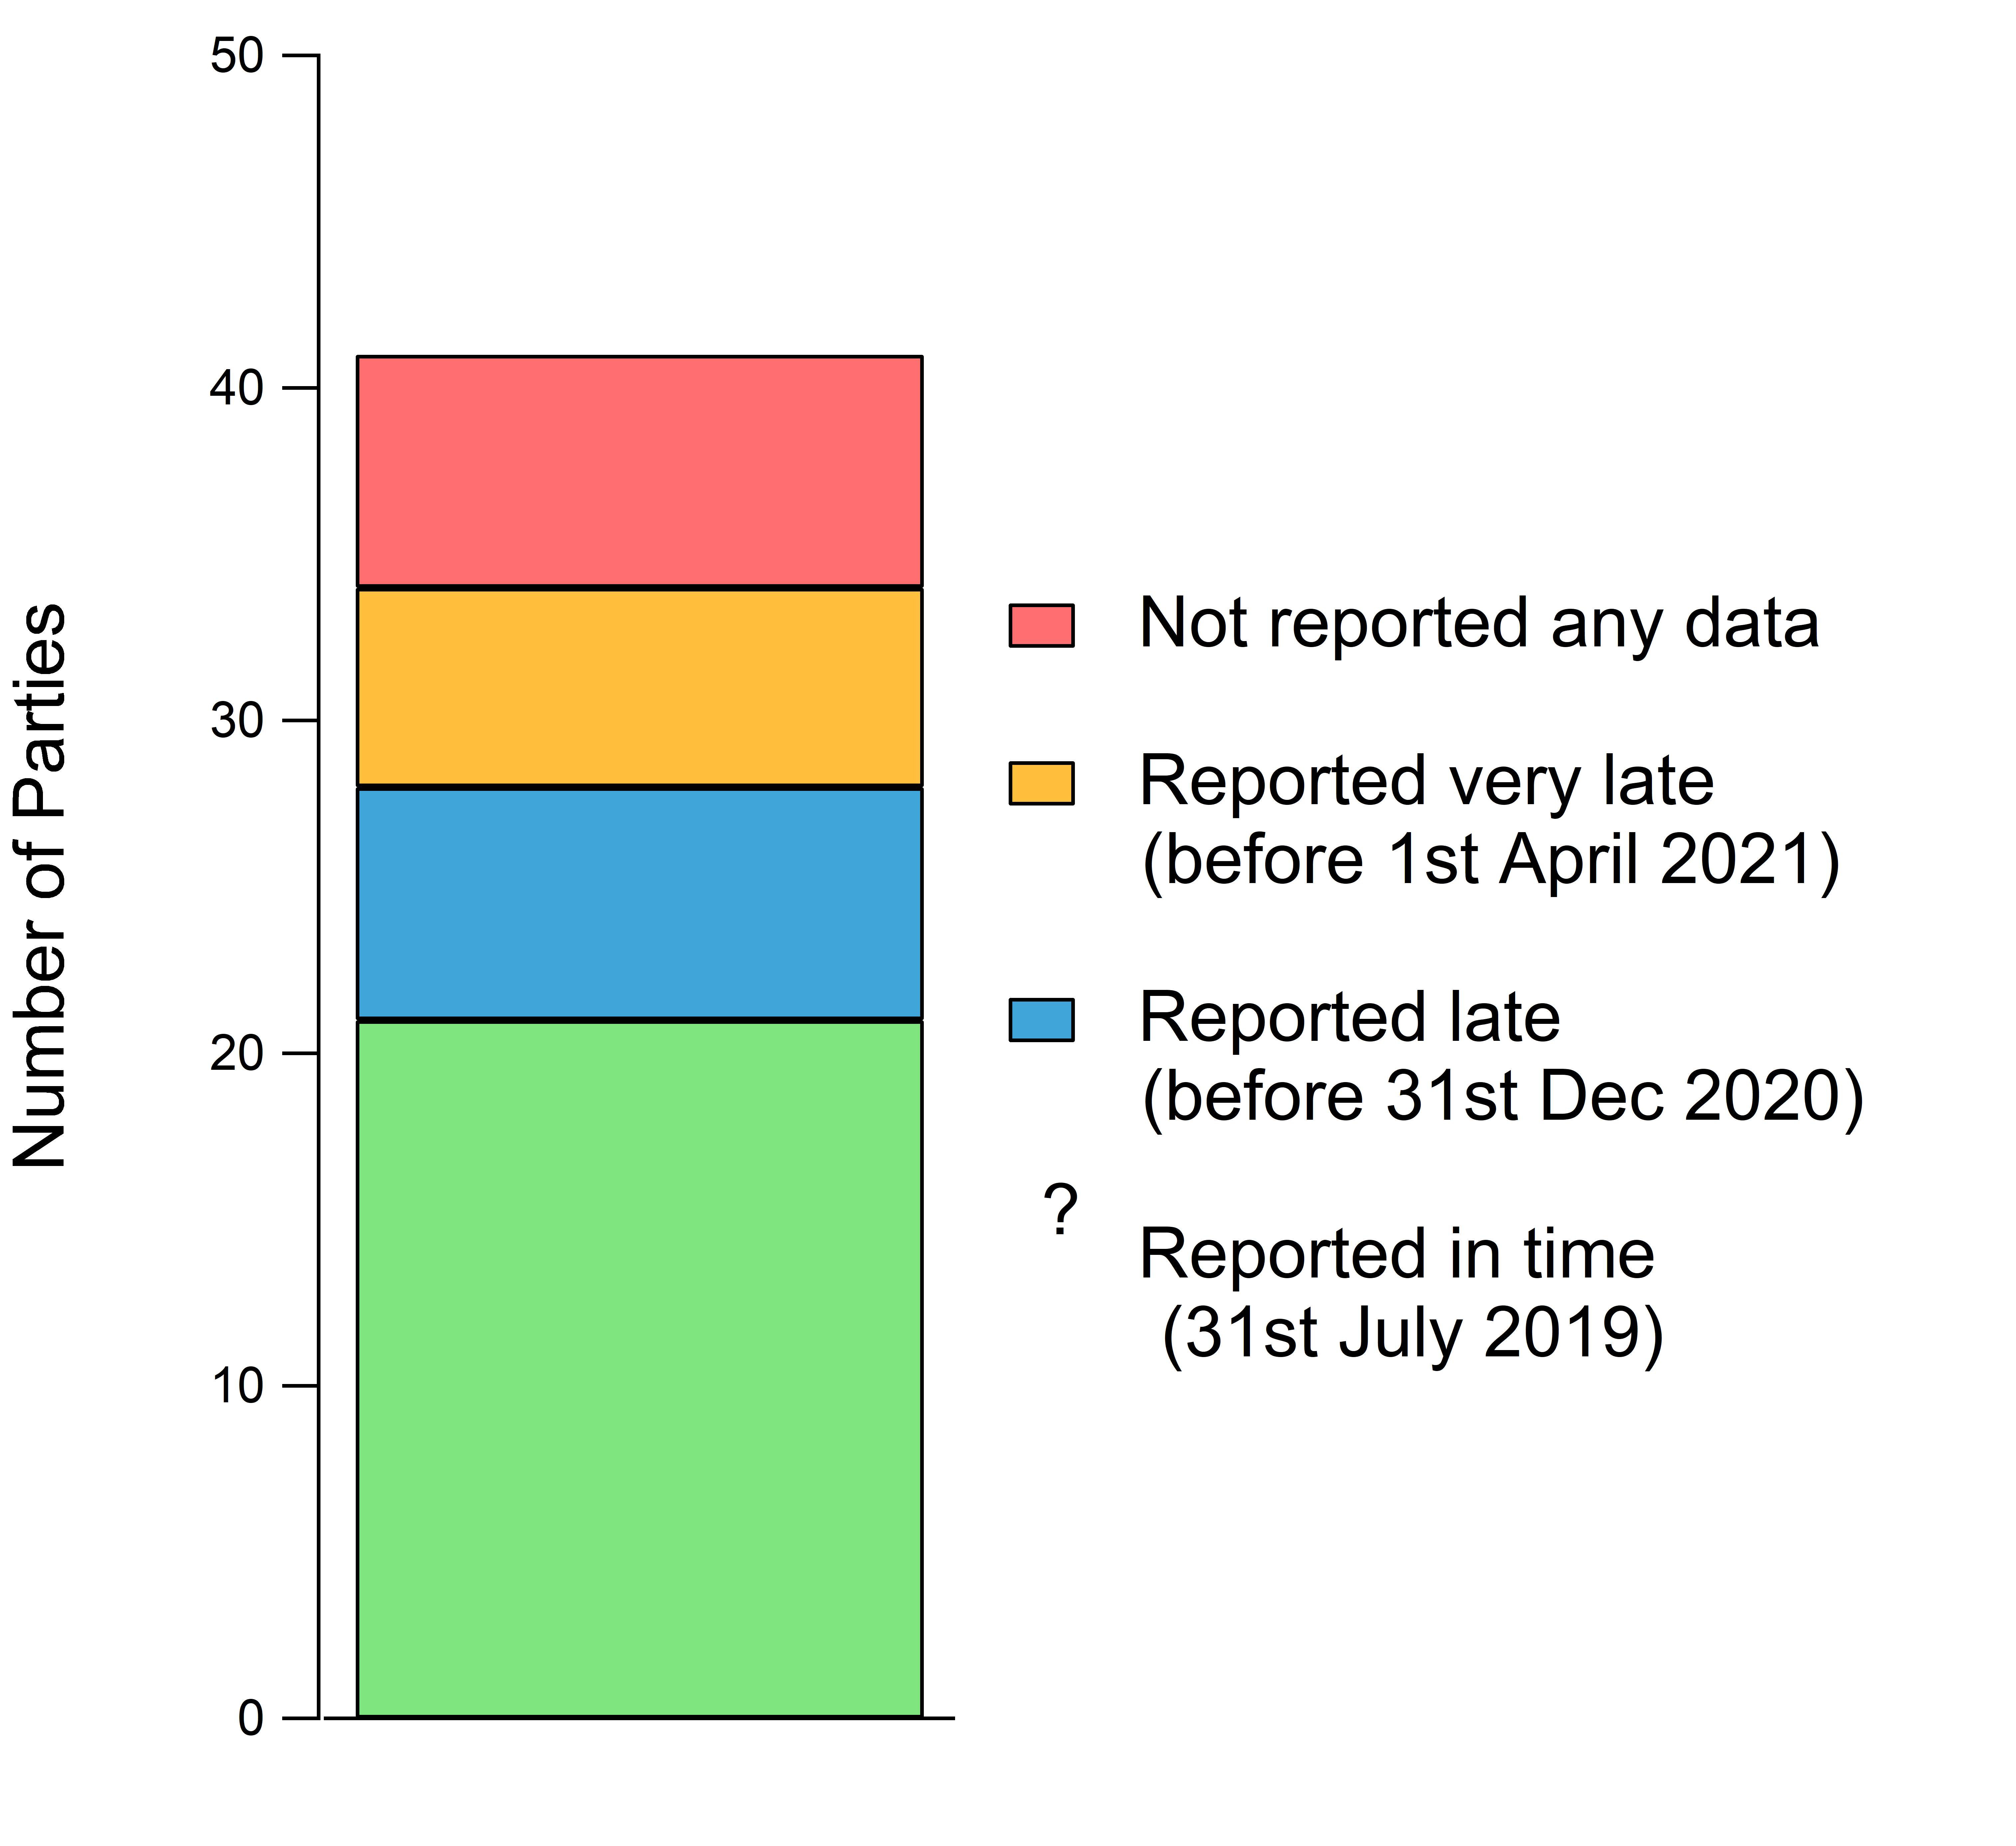
\includegraphics[width=0.45\paperwidth]{FIGS_Obs/reported.png}
\caption{\label{fig:Submission}Submission of 2019 data to EMEP/CCC.}
 \end{figure}

An online data submission and validation tool (\url{http://ebas-submit-tool.nilu.no}) was developed in 2016 improve  the timeliness and quality of the data reporting. The tool is designed to give the data submitters direct feedback on the formatted NASA Ames files, and suggestions on how to correct the files.  The format checker is directly linked to all (approx. 40) data format templates located at \url{http://ebas-submit.nilu.no/}, and it  is continuously being improved and updated, after feedback from the users or when new templates are developed. 

The requirement of checking the data files using the submission tool has significantly improved the correctness in the data files submitted, but still there are Parties not using the submission tool and report by e-mails. EMEP/CCC strongly encourage all the Parties to use the submission tool, which in fact is mandatory for submitting all the data to EMEP, unless otherwise have been agreed upon. In the coming years there will be further focus on improving the data submission tools to make it easier for the data provider to report correct and consistent data. 

The EMEP data are extensively used. In 2009, a user statistic was implemented for the EBAS database infrastructure.  
The statistic counts how much data are downloaded, displayed or plotted. Figure~\ref{fig:downloads} shows the access requests for EMEP data per year (about 300 thousand annual datasets). There was a big jump in 2013. This was the year when an automatic system for distributing all the data in EBAS to specific users was implemented. The number of downloads increased in 2020 compared to 2019. 

\begin{figure}[h]
\centering
\includegraphics[width=0.6\paperwidth]{FIGS_Obs/downloaded.png}
\caption{\label{fig:downloads}Access of EMEP data, number of annual dataset (compounds) per year.}
 \end{figure}

There is ongoing work to make the  access of data even more flexible to meet several of the user needs. In example using other platforms, like THREDDS (\url{https://thredds.nilu.no/thredds/catalog/ebas/catalog.html}) where NetCDF files are extracted from EBAS allowing faster access and the possibility to create more individual specific defined outputs for plotting, statistics, aggregates etc. Further implementing primary DOI for data in EBAS are also being developed. The development of the database infrastructure is inline with the FAIR principles (findable, accessible, interoperable and reusable).

\clearpage
\bibliographystyle{copernicus}         % change bibliography-name after each
\renewcommand\bibname{References}      % bibliographystyle command!
\addcontentsline{toc}{section}{References}
\bibliography{Refs,EMEP_Reports}
